%!TEX root = main.tex
\chapter{Filter}
\label{chap:filters}


\begin{figure}[H]
	\begin{center}
		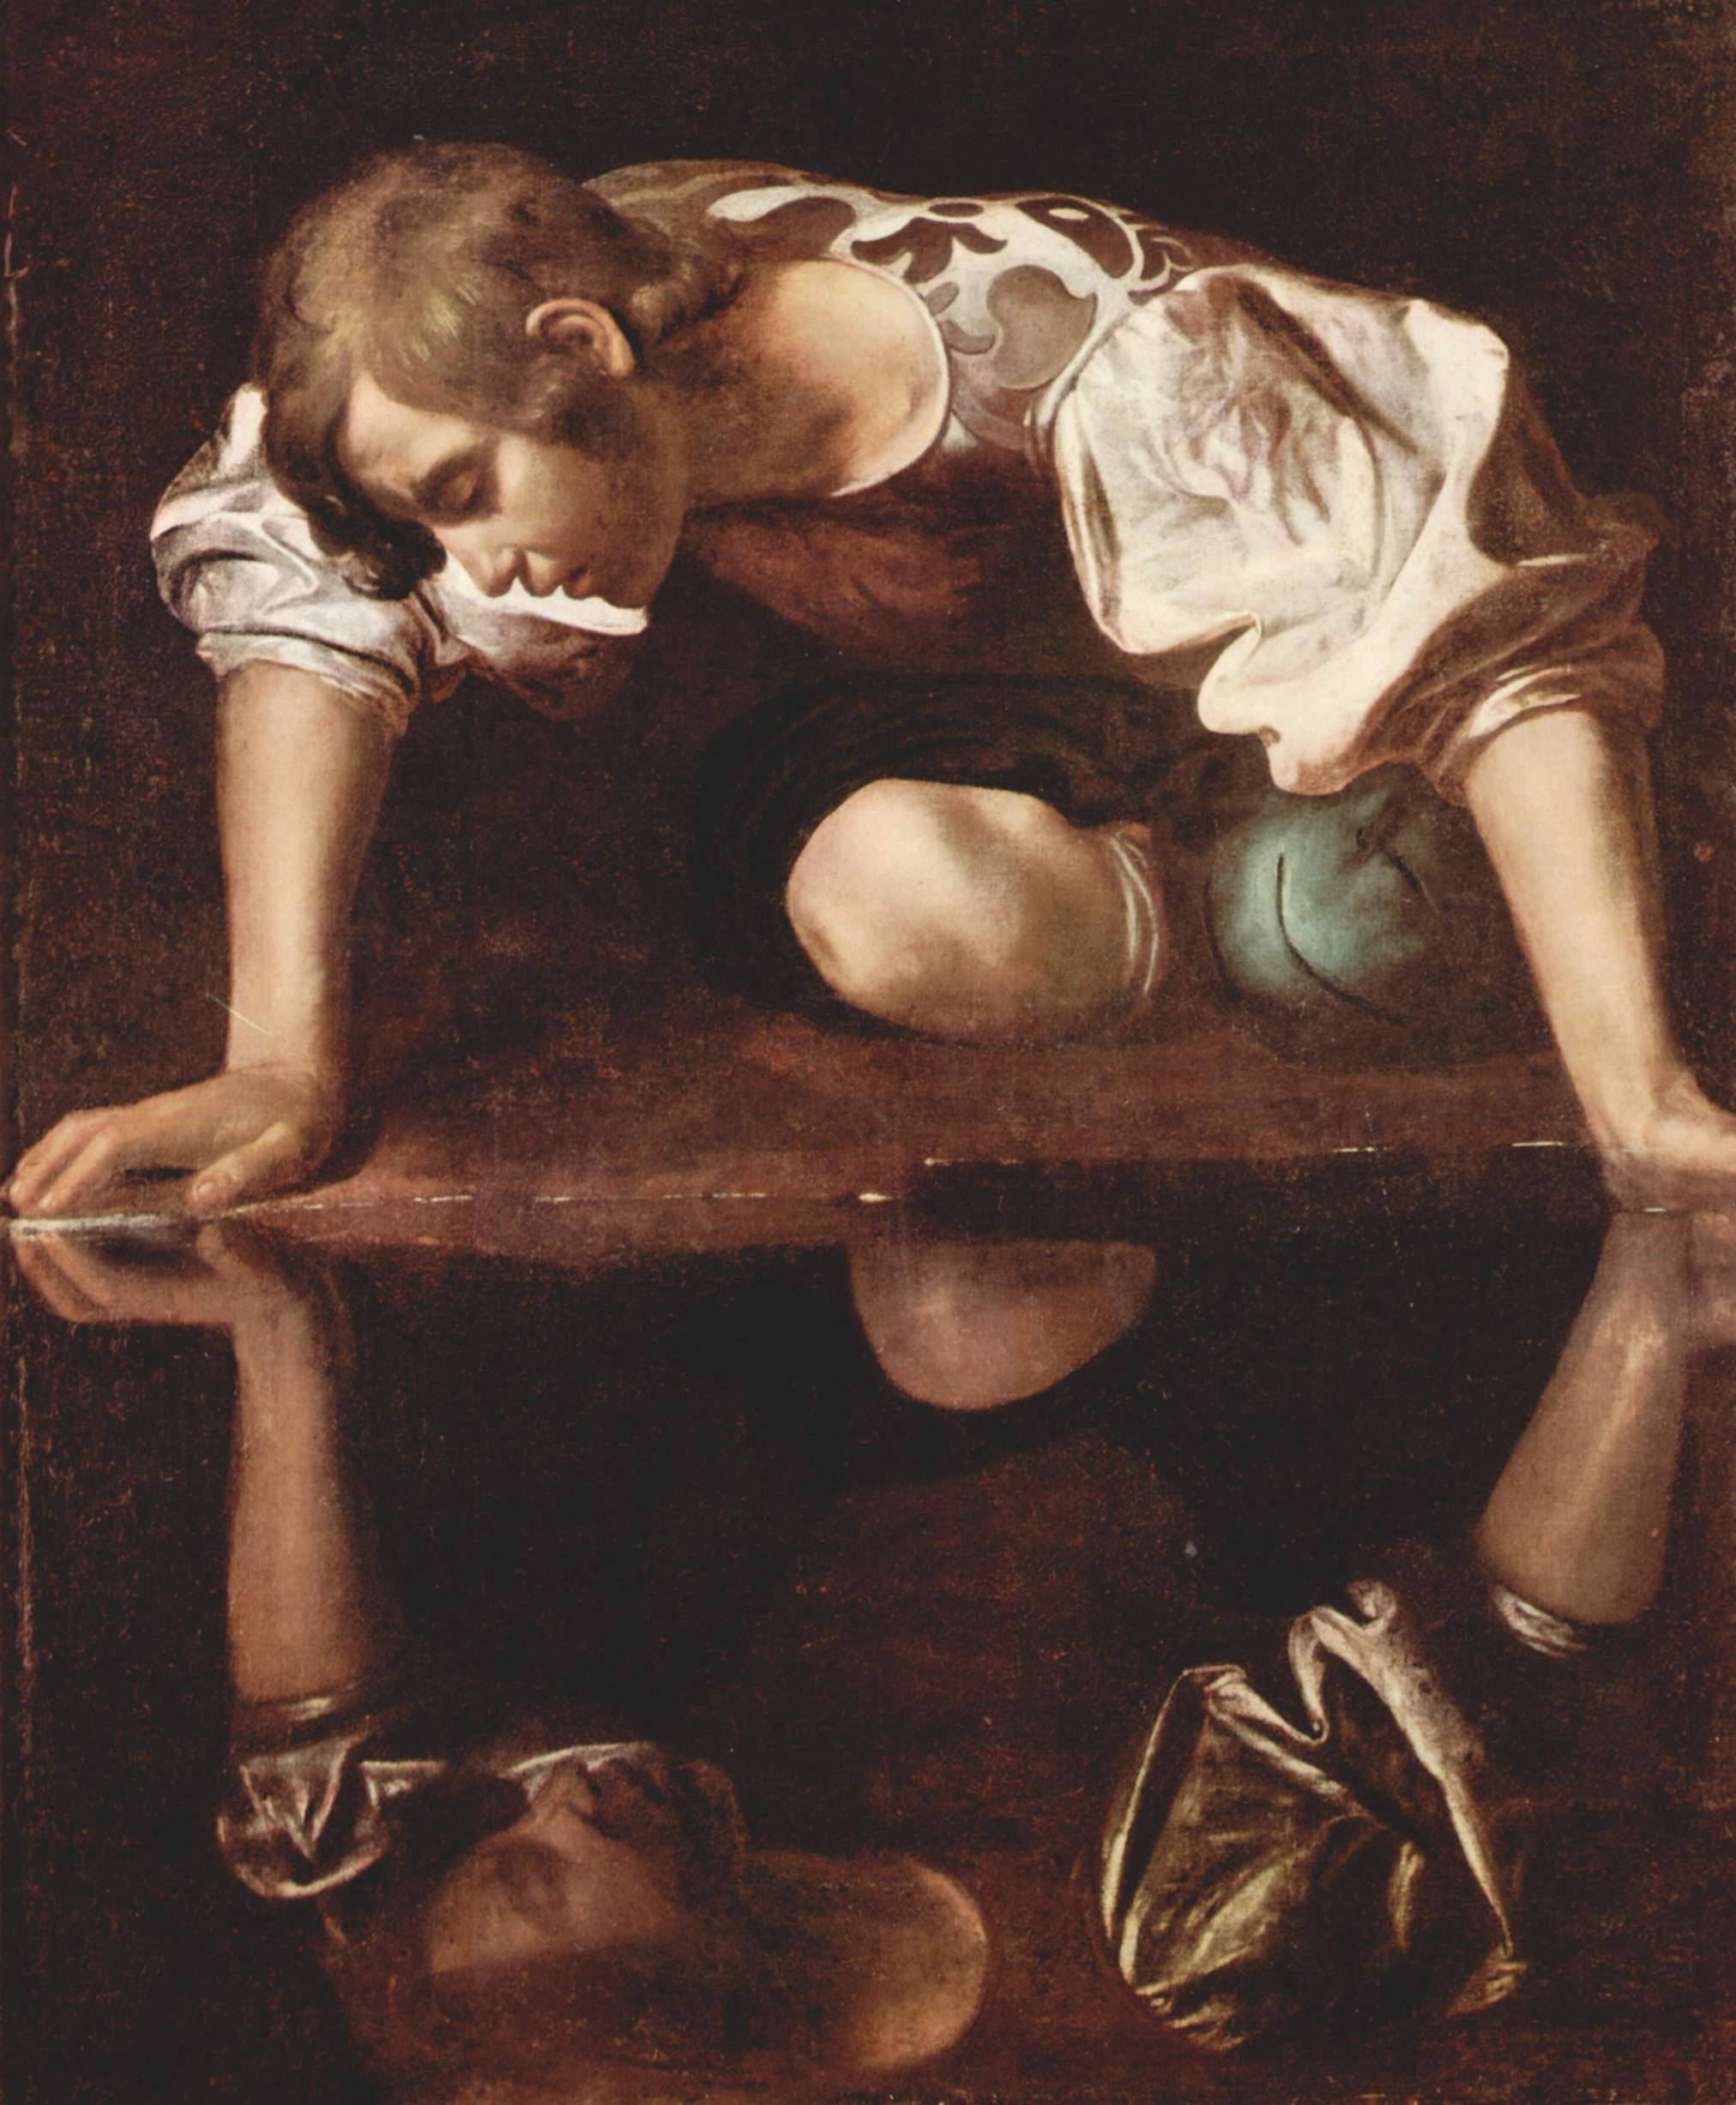
\includegraphics[width = 14cm]{img/Narciss_Caravaggio.jpg}
		\caption{Caravaggio, Narziss. ad Feedback: Echo liebt Narziss etc.}
		\label{fig:name}
	\end{center}
\end{figure}



\comm{lecture mind map missing}


What is a filter? We use filters a lot. We often need to shape the spectrum of a signal. Be it for technical reasons (DC-Offset removal, Anti-aliasing filters, crossovers, interpolation, ...) or for aesthetical ones (EQ-ing, subtractive synthesis)\\
Please take a moment and seriously ask yourself, knowing what you know about signals, knowing what we can do with a computer: How do we actually do this? What is a digital Filter? This is what this chapter will try to explain.\\

\section{Riddle and Getting a Feel for Filtering}

Three Questions in order to make you think about signals:


\begin{question}
	Please look at the image below. Can you draw an approximation of its spectrum? What signals could have been mixed to obtain this result?
% subsection raetsel (end)
\begin{figure}[H]
	\begin{center}
		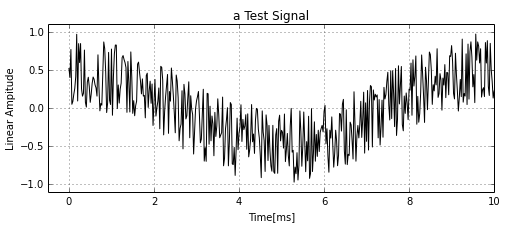
\includegraphics[width = 14cm]{raetsel_original.png}
		\caption{Original Signal}
		\label{fig:originalSignal}
	\end{center}
\end{figure}
\end{question}


\begin{Answer}
You should be able to see that there is a sinusoidal component in the signal. This sinusoid has a period of 10 ms, so a frequency of 100 Hz. But also you should see that it is not a clean sine wave, there is some noisy component in there. This is what you should have been able to infer from the image. In fact it is an (attenuated) 100Hz sinusoid mixed with (attenuated) white noise.
\end{Answer}


Woraus könnte das signal in Bild ~\ref{fig:originalSignal} bestehen?
\textbf{Kann jemand das spektrum aufmalen?}
% subsection raetsel (end)
\begin{figure}[H]
	\begin{center}
		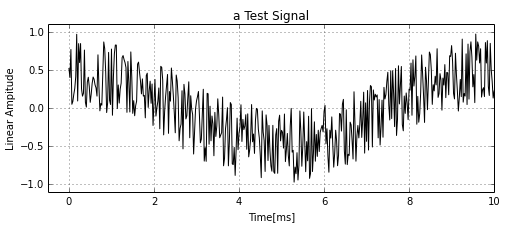
\includegraphics[width = 14cm]{raetsel_original.png}
		\caption{Original Signal}
		\label{fig:originalSignal}
	\end{center}
\end{figure}

Das Signal in Bild ~\ref{fig:originalSignal} wurde gefiltert und das Signal in Bild ~\ref{fig:raetsel_1} ist entstanden. Was für ein Filter wurde möglicherweise verwendet?

\begin{figure}[H]
	\begin{center}
		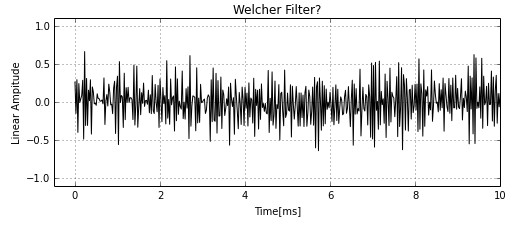
\includegraphics[width = 14cm]{raetsel_highpass.png}
% Notizen aus erster UE:\\
% Viellt. mit IR anfangen?
% Vielleicht davor noch: das beispiel mit noise + sinus.

% IR, bypass system, hall system.

% garnicht faltung. Moving average zu long FIR.
% Impuls antworten anhand beispielen besprechen.


% \begin{enumerate}
% 	\item FIR!

% kammfilter(FF)

% dann FIR kammfilter

% chorus
% flanger

% LFO

% ->index/tiefe, offset, frequenz wdh.


% -frequenzgang
% ausl\"oschungen, rechnen..

% \item 
% FIR one sample delay\\

% FIR bauen, vllt. an tafel blockdiagramm.\\

% FIR hipass\\


% \item 

% mehrere Samples delay
% IR
% differenzen gleichung

% eventuell Faltung(faltungs hall connection herstellen)

% faltung als multiplikation d. spektra
% multiplikation als faltung d spektra.

% M4L faltungs hall herzeigen

% LTI?

% differentiator, akkumulator?

% \item
% IIR\\



% notizen POlyphonie
% was separat, was einmal

% \end{enumerate}

% \section{einfuehrung} % (fold)
% \label{sub:einfuehrung}


% Ziel der LV:\\
% \begin{enumerate}
% 	\item Gefühl dafür bekommen was die häufigsten Operationen der DSV eigentlich tun.
% 	\item Gefühl dafür bekommen, dass es günstig ist, zwischen verschiedenen repräsentationen hin und her zu wechseln (time und frequency domain, aber auch system repräsentationen)
% 	\item Sich in professioneller literatur(DSP lehrbücher) nicht völlig verloren fühlen.
% 	\item schönheit zu sehen dass alles das \glqq{}gleiche\grqq{} ist.(Delay, filter, reverb, chorus, flanger etc)
% \end{enumerate}

% Wozu?:\\
% \begin{enumerate}
% 	\item Wir arbeiten ständig mit Operationen der DSV. Filter sind nicht nur in synthesizern. Ein tieferes verständnis erleichtert die arbeit. Wie funktioniert zum beispiel ein blur?
% 	\item Was ist ein FeedForward compressor?
% \end{enumerate}


% Nachdenken über filter allgemein. Was ist ein filter im gespür d. studenten. \\
% Bekannt was ein LTI system ist?\\

% \subsection{Raetsel} % (fold)
% \label{sub:raetsel}

% 		\caption{raetsel 1}
% 		\label{fig:raetsel_1}
% 	\end{center}
% \end{figure}

% Das Signal in Bild ~\ref{fig:originalSignal} wurde gefiltert und das Signal in Bild ~\ref{fig:raetsel_2} ist entstanden. Was für ein Filter wurde möglicherweise verwendet?


% \begin{figure}[H]
% 	\begin{center}
% 		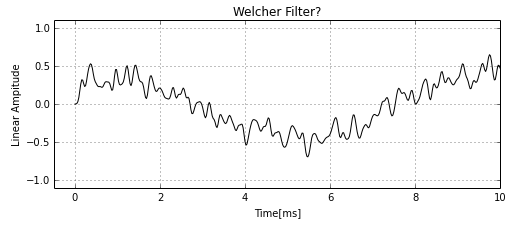
\includegraphics[width = 14cm]{raetsel_lowpass.png}
% 		\caption{raetsel 2}
% 		\label{fig:raetsel_2}
% 	\end{center}
% \end{figure}

% \newpage
% \subsubsection{Lösung} % (fold)
% \label{sub:l_sung}

% % subsection l_sung (end)
% Original signal = White noise + cosinus bei 100 Hz.\\
% Raetsel 1 : ein Highpass.\\
% Raetsel 1 : ein Lowpass.\\
% (many FIR filters in series.)





% \newpage
% -Wie könnte ein filter realisiert werden?\\
% -Ein digitales signal ist eine reihe von zahlen, eine sequenz von werten. (über bildliche darstellungen sprechen)\\
% -Echtzeit fall: ich bekomme in ein system ein signal(also ständig werte) und soll ein zb. lowpass gefilteretes signal ausgeben.\\
% \textbf{Was kann ich mit dem signal machen? Zum beispiel addieren, multiplizieren, verzögern.}\\


% Einfacher moving average. Zunächst nur an der tafel!
% Impulsantowrt ausrechnen!
% Was ist ein impuls.\\
% Was ist eine impulsantwort? Beispiele.. untit impulse ( = dirac impuls, dirac gunktion, delta function)\\

% Diagramm aufmalen:

% impuls \(\rightarrow\) Raum \(\rightarrow\) Impulsantwort\\
% oderr \\
% impuls \(\rightarrow\) beliebiges system \(\rightarrow\) Impulsantwort\\
% \textbf{anwendugsbeispiel:} tontechnik bei okto; mischpult ausmessen, dbmax ausmessen(fragwürdige sache! Wieso?)




% \textbf{FRAGE}\\
% Ein system(zB. ein Filter) hat folgende Eigenschft:\\
% Wenn zwei signale getrennt (d.h. unabhängig voneinander, zB. nacheinander.) in das system geschickt werden, und die Ergebnisse summiert werden, entsteht das signal \(P\). Wenn andererseits die signale zuvor summiert werden und dann in das system geschickt werden entsteht ebenfalls \(P\). Welche gleichung etspricht einer beschreibung dieser eigenschaft?



% \begin{enumerate}
% 	\item \(f(x)+f(y) = f (x * y) = P\)
% 	\item \(f(x)+f(y) = f (x + y) = P\)
% 	\item \(f(x)+f(x) = f (x + y) = P\)
% 	\item \(f(x)+f(y) = f (x + x) = P\)
% 	\item nichts von alledem.
% \end{enumerate}

% \newpage
% richtig : nr.2 \\
% \\

% Erklärung eines LTI systems:

% \begin{itemize}
% 	\item Linear:
% 		\begin{itemize}
% 			\item Superpositionsprinzip \(f(x)+f(y) = f (x + y)\)
% 			\item Homogenität \(a*f(x) = f(a*x)\) 
% 		\end{itemize}
% 	\item Time Invariant (zeit-invariant)
% \end{itemize}


% Zurück zu filter: 
% was glauben sie wie er funktioniert. \\
% \\

% \section {kammfilter}

% Wiederum fragen was sich die studenten vorstellen.\\


% \glqq{}Wir bauen ein delay.\grqq{}
% nicht vergessen: block~, subpatcher.


% \begin{figure}[h]
% 	\begin{center}
% 		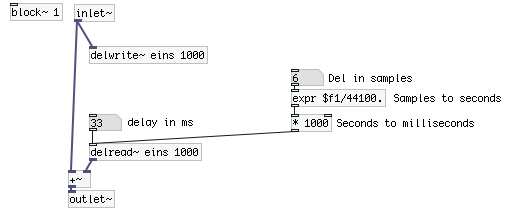
\includegraphics[width = 14cm]{simpleDelay.png}
% 		\caption{SimpleDelay}
% 		\label{fig:simpleDelay}
% 	\end{center}
% \end{figure}

% Studenten sollen ausprobieren. Verschiedene inputs f. kammfilter. \\

% Modulation des kammfilters. Studenten sollen LFO an den kammfilter dran bauen.\\
% \(\rightarrow\) Flager \\
% \(\rightarrow\) Chorus \\

% \textbf{index/tiefe, offset, frequenz wiederholen.}


% \begin{figure}[h]
% 	\begin{center}
% 		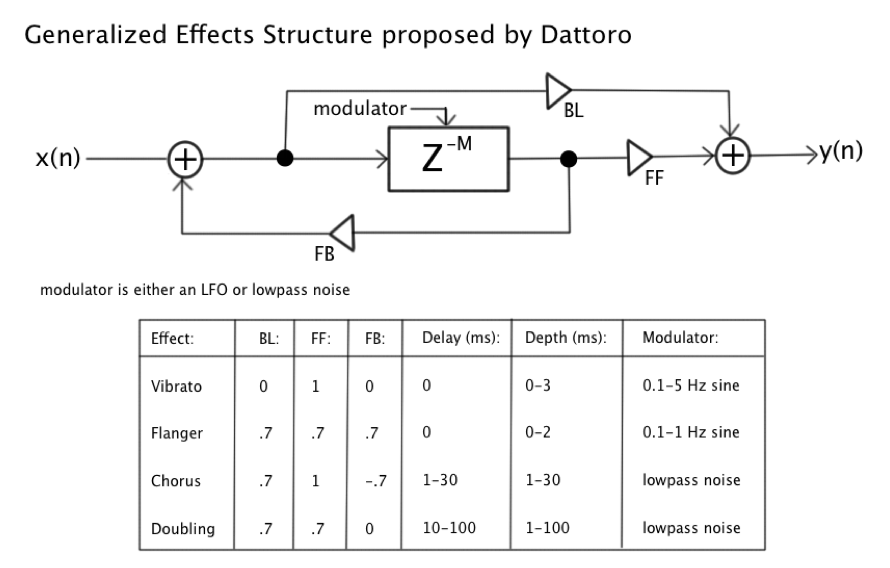
\includegraphics[width = 14cm]{generalizedEffect.png}
% 		\caption{generalized Effect structure}
% 		\label{fig:genEffect}
% 	\end{center}
% \end{figure}

% über name sprechen, sowohl spectrum als auch Impulsantwort(IIR variante) sind kammförmig. \\
% Eigentlich einfach ein delay, ein delay mit feedback im falle von IIR.\\




% \begin{figure}[h]
% 	\begin{center}
% 		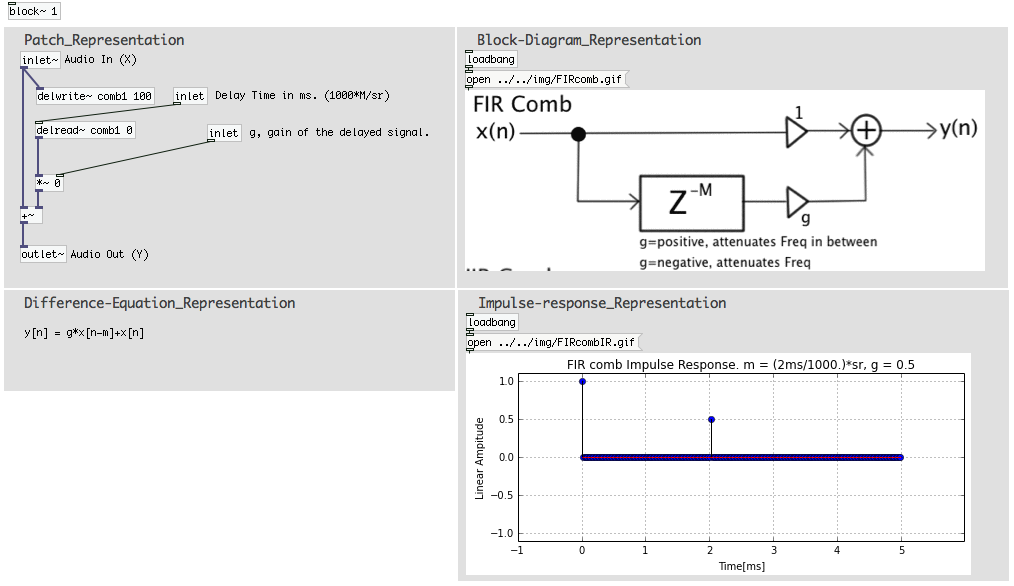
\includegraphics[width = 14cm]{img/combFIR_patch.png}
% 		\caption{Der Patch 01\_combFilter.pd}
% 		\label{fig:01_combFilter}
% 	\end{center}
% \end{figure}



% Zunächst nicht wichtig die versch. representationen zu verstehen. \\
% Patch representation kurz durchbesprechen. Sollte verständlich sein.\\

% Unterschiedliche representationen durchbesprechen.
% Fragen, abstimmen?, was die studenten für die angenehmste representation halten.



% \begin{itemize}
% 	\item Patch: vorteile: interaktiv, allgemein, reinfolge der events nachvollziehbar. Nachteil: nicht sehr übersichtlich. Nicht sehr konzis, nicht kompakt.
% 	\item Block Diagramm: übersichtlich, allgemein. Reinfolge der events klar, pfeile! Fluss, richtung, eindeutig. Nachteile: Nicht kompakt.
% 	\item differenzen gleichung: Vorteil: kompakt, konzis. Nachteil: reinfolge der events nicht klar ersichtlich: kein rezept, eher eine beschreibung. (nicht imperativ sondern deklarativ, va. im Fall von Feedback)
% 	\item Impulsantwort: \textbf{Frage: was ist ein Impuls?}  Vor/Nachteil: Nicht allgemein, nur ein spezieller zustand des systems beschrieben. Nicht kompakt, aber kann sehr intuitiv sein. Beispiele an tafel: IR von bypass-system, IR mit viel hall, IR von bandpass filter mit hoher resonanz, eventuell: differentiator, accumulator.
% 	\item andere representationen: text-code, transfer funktion, frequency response(magnitude + phase response/group delay)
% \end{itemize}




% \newpage


% \section {Moving Average}

% \textbf{Wo hat der kammfilter immer sein erstes Tal im spectrum?}
% Sinus an tafel malen.
% Antwort:
% bei 

% \(\lambda =  (2* \Delta t) \)
% (wobei \(\Delta t\) die delay zweit in sekunden. und \(\lambda\)  die periodendauer der gesuchten frequenz.) Daher:\\
% \(
% f_c = 1/(2* \Delta t)
% \)

% Nun wird das delay auf ein sample reduziert. Ein lowpass entsteht der seine grenzfrequenz bei sr/2 hat.\\

% Frage: was macht ein lowpass filter in der timedomain?


% \begin{figure}[h]
% 	\begin{center}
% 		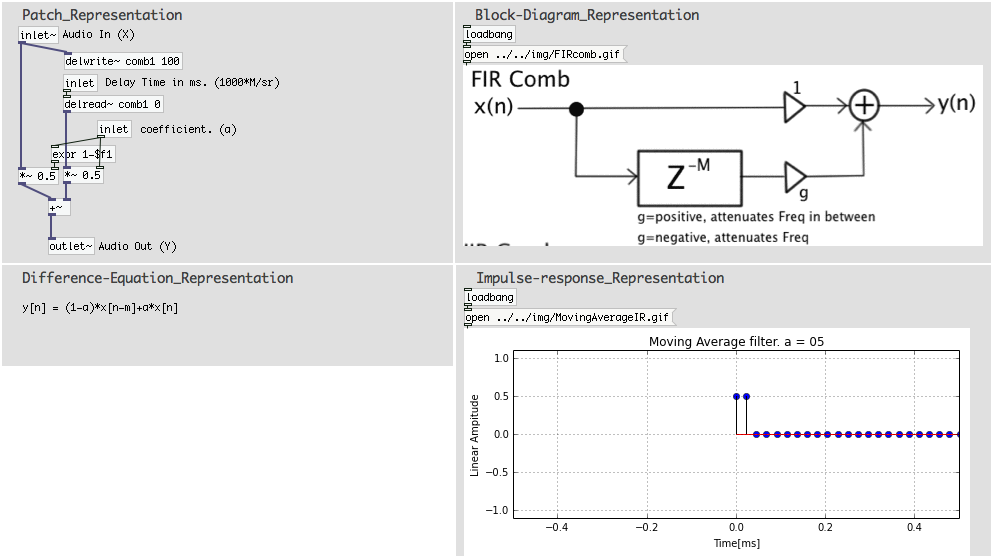
\includegraphics[width = 14cm]{movingAverage.png}
% 		\caption{movingAverage}
% 		\label{fig:movingAverage}
% 	\end{center}
% \end{figure}


% \textbf{EXKURS: VIDEO FILTER, lowpass, time domain erkennen.}


% \newpage
% \textbf{Frage:} Vergleiche original und die gefilterte variante (01.mov) . Was für ein filter könnte angewandt worden sein:
% \begin{enumerate}
%  	\item lowpass
%  	\item bandpass
%  	\item hipass
%  	\item notch
%  	\item nichts von alledem
%  \end{enumerate} 


% wie könnte ein highpass realisiert werden? Wie schaut der effekt eines highpass filters in der frequenz- und wie in der timedomain aus?


% \section{convolution, Faltung}

% Video (unten) zeigen, vorher erklären: \\

% conv theorem.

% http://youtu.be/\_vyke3vF4Nk?t=25m16s \\
% start bei min 25.

% \textbf{maxpatch}




% %%--------------------------------------------------------------------------
% %% IIR/FIR
% %%--------------------------------------------------------------------------
% \section {IIR/FIR}

% Je steiler die Filterflanke sein, je komplexer der filter sein soll, desto mehr delays werden benötigt.\\

% Wieso: einfache Erklärung: Um aus einem signal, das alle frequenzen enthält (zB dirac impuls) ein signal zu machen, das hauptsächlich sehr tiefe frequenzen enthält wird ein system benötigt das \glqq{}lange wellen\grqq{} zu produzieren im stande ist. 

% An tafel zeichnen: dirac impuls und unit step/ DC. Frage nach spectrum.\\

% frage nach FIR der diesen IR haben könnte.

% \textbf{Patch: lomgSimpleFir}

% Grenzfall: integrator macht aus unit impulse, \(delta [n]\), unit step signal\(u[n]\)(DC).

% Integrator an tafel malen.\\

% Daher:
% Es kann gezeigt werden dass ein feedback pfad einer unendlichen menge an delays gleichkommt, siehe IR.

% \textbf{Patch: 02\_combFilterIIR}

% nebenbei:
% linear phase = symmetrischer IR, immer FIR, daher weniger performant.
% Linear phase filter sind notwendig wenn die timedomain wellenform möglichst unbeeinträchtigt bleiben soll.

% \subsection{Onepole} % (fold)
% \label{ssub:onepole}

% % subsubsection subsubsection_name (end)
% onepole an tafel beschreiben. Block diagramm, malen, nach differenzengleichung fragen. Patch herzeigen.\\

% \textbf{patch: IIRtest} \\
% danach:\\
% \textbf{patch: IIRtest2} \\

% Fragwürdig aber falls interesse:
% onepole coeff berechnung zB:\\

% \begin{equation}
% a_0 = \frac{2 \pi f_c} {sr}
% \end{equation}

% oder

% \begin{equation}
% a_0 = sin(\frac{2 \pi f_c} {sr})
% \end{equation}


% \section{Hausübung}

% hausübung: Baue einen einen chorus. TESTSIGNAL AUSBESSERN! nicht noise!!

